\chapter{Avaliação Experimental}
% explicar objetivos da avaliação experimental.
\section{Ambiente computacional}
Para os experimentos realizados neste trabalho, foram utilizados 2 máquinas com configrações diferentes de hardware. Um deles possui o \textit{hostname} poseidon e é hospedado nas dependências do Laboratório de Arquitetura de Computadores e Microeletrônica (LAM), enquanto o outro trata-se de um notebook pessoal com \textit{hostname} jvdvostro. O servidor poseidon foi utilizado para realizar a busca de hiperparâmetros, pois é a etapa que mais consome recursos computacionais. O jvdvostro foi utilizado para coletar as métricas de inferência, gerar gráficos e fazer a análise dos resultados. A Tabela~\ref{tab:hardware} expõe as configurações de \textit{hardware} de ambos computadores utilizados nos experimentos.

\begin{table}[!htp] \label{tab:hardware}
    \caption{Configurações de \textit{hardware} dos computadores.}
    \setlength\extrarowheight{5pt}
    \centering
    \begin{tabular}{|c|c|c|c|}
        \hline
        \rowcolor[HTML]{C0C0C0}
        Hostname  & CPU                           & RAM   & Sistema Operacional \\ \hline
        jvdvostro & Intel i7-5500U (4) @ 3.000GHz & 8 GB  & Arch Linux x86\_64  \\ \hline
        poseidon  & Intel i7-6700 (4) @ 3.40GHz   & 32 GB & Ubuntu Linux        \\ \hline
    \end{tabular}
\end{table}

Os experimentos foram realizados utilizando \textit{scripts} e \textit{notebooks} Python, dependendo da etapa e da finalidade. Para a busca de hiperparâmetros e avaliação dos modelos em relação ao erro, foram utilizados \textit{scripts}, enquanto para a avaliação de métricas de tempo de inferência e uso de memória foram utilizados \textit{notebooks}.

\section{Coleções de dados}
Foram utilizadas para os experimentos deste trabalho 3 coleções de dados. Dentre estas, duas foram coletadas de fontes públicas abertas na internet e uma foi gerada artificialmente. Todas foram armazenadas em disco local no formato tabular com extensão CSV. O número de casos confirmados de Covid19 no Rio de Janeiro foi o primeiro dataset utilizado nos experimentos e serviu um dos motivadores do estudo realizado. A temperatura mínima diária em Melbourne e os dados gerados sintéticamente serviram como prova de conceito para averiguar a eficiência dos métodos aplicados em diferentes cenários, portanto foram submetidos aos mesmos métodos e técnicas aplicados na primeira coleção de dados. As duas coleções de dados retiradas de fontes públicas possuem licensa que permite a sua utilização para fins acadêmicos, e podem ser consultadas nos endereços disponibilizados nesta Seção.

\subsection{Casos confirmados de Covid19 no Rio de Janeiro} \label{subsec:casos_confirmados}
Com o auxílio da biblioteca \textit{requests} do Python, foi criado um \textit{script} para baixar e armazenar localmente o número de casos confirmados de Covid19 no Estado do Rio de Janeiro. O arquivo csv foi baixado diretamente do web site da Secretaria de Saúde do Estado do Rio de Janeiro. \footnote{$http://sistemas.saude.rj.gov.br/tabnetbd/dhx.exe?covid19/covid_munic_diario.def$} Para manter a reprodutibilidade dos experimentos, o período analisado foi congelado entre as datas 01/01/2020 e 04/07/2021. A Figura~\ref{fig:casos_confirmados} mostra um gráfico da série temporal não acumulada do número de casos confirmados diário, ou seja, os valores absolutos de casos registrados em cada dia sem considerar os dias anteriores.

\begin{figure}[!htp]
    \centering
    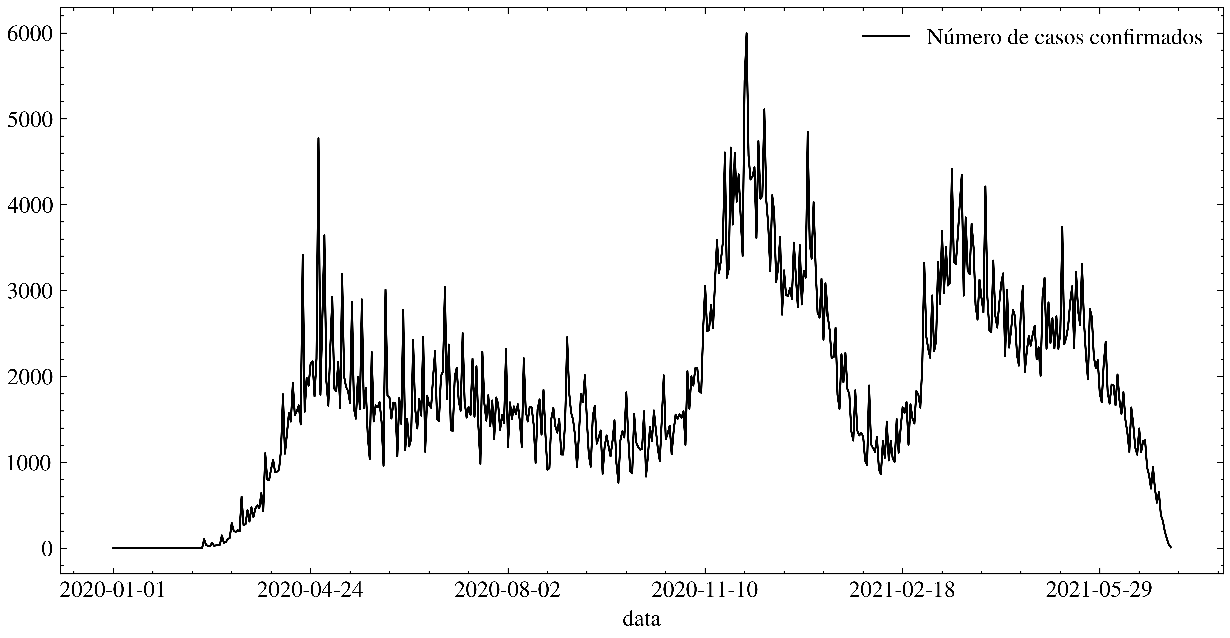
\includegraphics[width=5.0in]{img/casos_confirmados.pdf}
    \caption{Série temporal do número de casos confirmados de Covid19 no Rio de Janeiro.}
    \label{fig:casos_confirmados}
\end{figure}

A Figura~\ref{fig:casos_confirmados} mostra que há flutuações a curto pazo, que podem ter sido geradas por diversos fatores na coleta dos dados, como, por exemplo, a subamostragem. Como a coleta dos dados utilizados foi feita de fontes externas e públicas, os experimentos deste se limitaram a trabalhar com o dado como foi disponibilizado, sem aprofundar na avaliação da coleta. Porém, para remover a influência dessas flutuações, foi aplicado o método de médias móveis variando o parâmetro do número de amostras junto à busca de hiperparâmetros para encontrar o melhor ajuste. A Figura~\ref{fig:casos_confirmados_ma} mostra a mesma série temporal com as médias móveis em vermelho considerando-se o parâmetro $n=7$ como exemplo de suavização na flutuação dos valores da série temporal.

\begin{figure}[!htp]
    \centering
    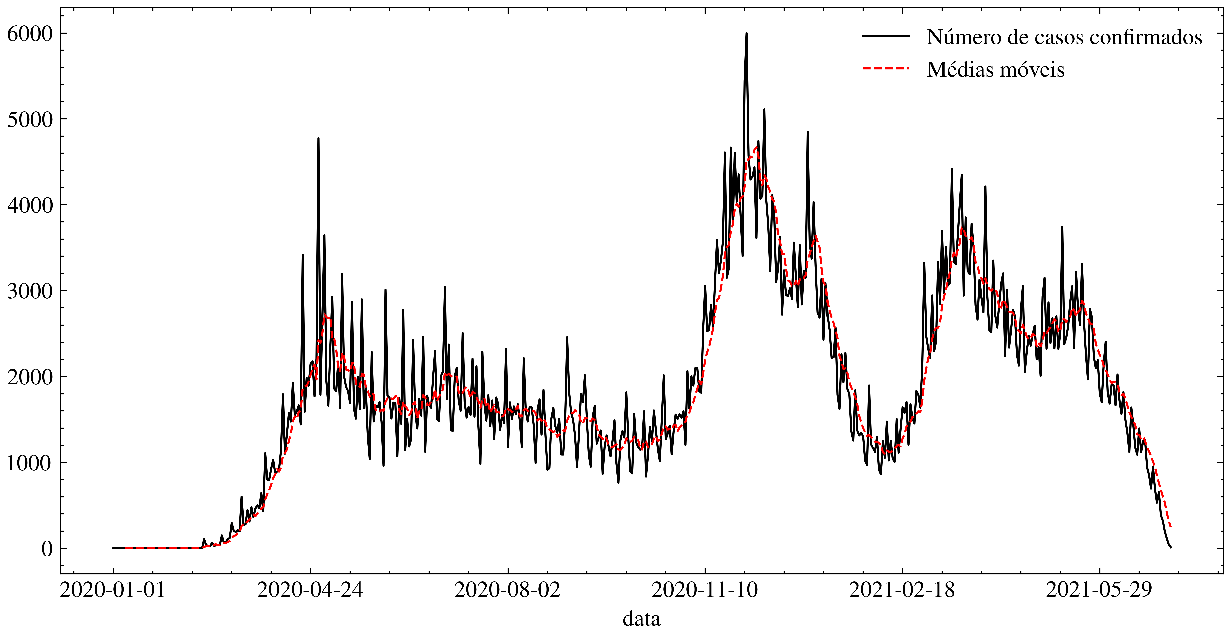
\includegraphics[width=5.0in]{img/casos_confirmados_ma.pdf}
    \caption{Médias móveis do número de casos confirmados de Covid19 no Rio de Janeiro.}
    \label{fig:casos_confirmados_ma}
\end{figure}

\FloatBarrier

\subsection{Temperatura mínima diária em Melbourne}
Assim como na coleção de dados referente ao número de casos confirmados de Covid19 no Rio de Janeiro~\ref{subsec:casos_confirmados}, os dados de temperatura mínima diária em Melbourne foram baixados através de um \textit{script} Python com o auxílio da biblioteca \textit{requests}. O arquivo pode ser baixado diretamente do GitHub \footnote{$https://raw.githubusercontent.com/jbrownlee/Datasets/master/daily-min-temperatures.csv$} e também pode ser encontrado em um desafio do Kaggle \footnote{$https://www.kaggle.com/paulbrabban/daily-minimum-temperatures-in-melbourne$}.

\begin{figure}[!htp]
    \centering
    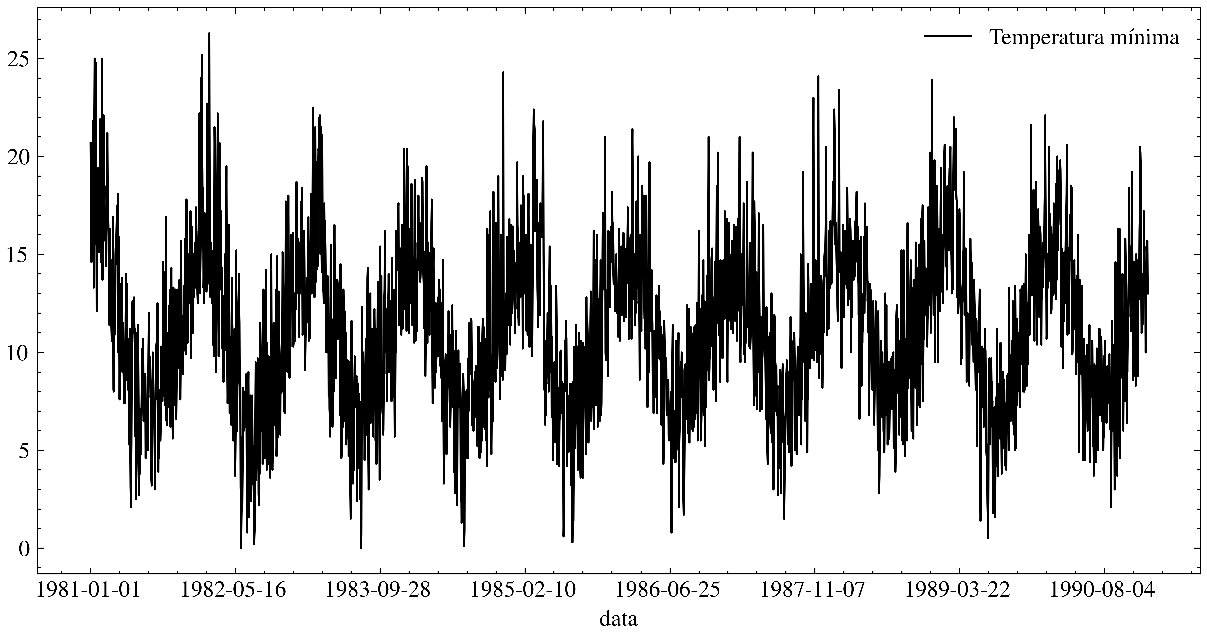
\includegraphics[width=5.0in]{img/temperatura_minima_diaria.pdf}
    \caption{Série temporal da temperatura mínima diária em Melbourne.}
    \label{fig:temperatura_minima_diaria}
\end{figure}

A Figura~\ref{fig:temperatura_minima_diaria} mostra que a quantidade de observações na série temporal da temperatura mínima diária em Melbourne é muito superior ao número de casos confirmados de Covid19, e correspondem ao período entre 01/01/1981 e 31/12/1990. Outro ponto divergente é a observabilidade do caráter sazonal com período de um ano. Porém, as flutuações de curto prazo permanecem, e continuam configurando um problema para o ajuste de modelos preditivos que precisam generalizar para realizar inferências mais acertivas.

\begin{figure}[!htp]
    \centering
    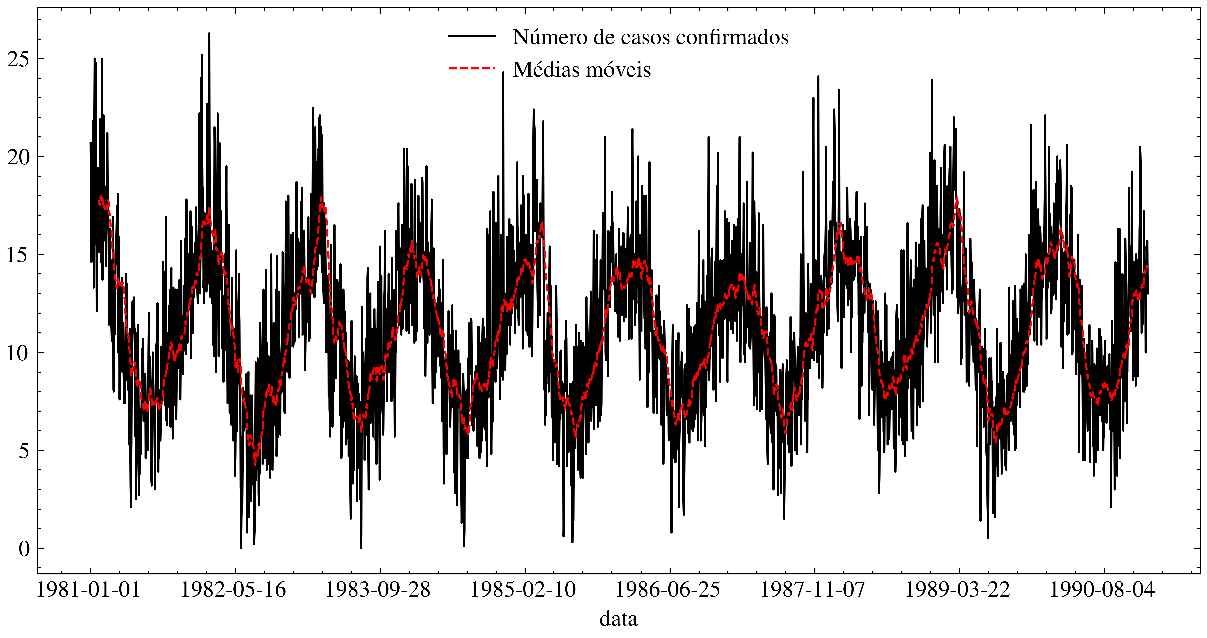
\includegraphics[width=5.0in]{img/temperatura_minima_diaria_ma.pdf}
    \caption{Médias móveis da temperatura mínima diária em Melbourne.}
    \label{fig:temperatura_minima_diaria_ma}
\end{figure}

A Figura~\ref{fig:temperatura_minima_diaria_ma} mostra as médias móveis da temperatura mínima diária em Melbourne em vermelho. O parâmetro utilizado para gerar esta figura foi $W=30$, que foi escolhido para representação gráfica por se tratar de uma série com aproximadamente um ano de período de sazonalidade.

\FloatBarrier

\subsection{Série temporal sintética}
Uma coleção de dados foi gerada de forma sintética com o auxílio da biblioteca \textit{numpy} do Python com características criadas artificialmente somando componentes como tendência, sazonalidade, ruído branco e fatores para distorção da estacionaridade seguindo o método apresentado em Yıldırım Soner, 2020 \cite{syntheticdata}. Essa série temporal é contruída com o objetivo de avaliar a capacidade de generalização dos modelos em cima dos componentes que estes costumam considerar como base, justificando a importância de ter sido gerada sinteticamente.

Em uma série temporal, a tendência é o padrão que evidencia o crescimento ou decrescimento dos valores a longo prazo. Portanto, para compor a série temporal sintética, foi considerada uma função linear crescente como fator de tendência. A Figura~\ref{fig:upward_trend} mostra a componente resultante gerada sinteticamente.

\begin{figure}[!htp]
    \centering
    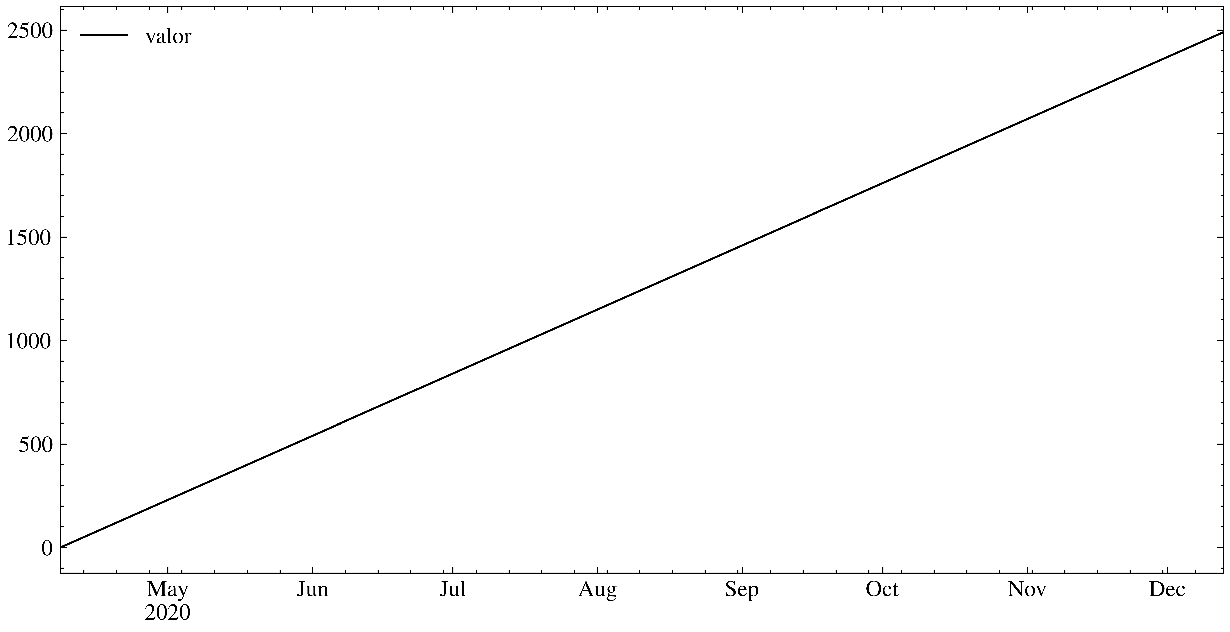
\includegraphics[width=5.0in]{img/upward_trend.pdf}
    \caption{Componente de tendência crescente.}
    \label{fig:upward_trend}
\end{figure}

A sasonalidade pode ser caracterizada pela presença de variações semelhantes que ocorrem em intervalos regulares de tempo. Então, para simular um comportamento sazonal, foi aplicado um crescimento cúbico seguido de um crescimento quadrático nos primeiros 50 dias, e então esse mesmo padrão foi repetido ao longo de toda a série temporal até o último dado observado. Na Figura~\ref{fig:seasonal_pattern} fica clara a repetição do padrão com as 2 curvas de crescimento seguidas.

\begin{figure}[!htp]
    \centering
    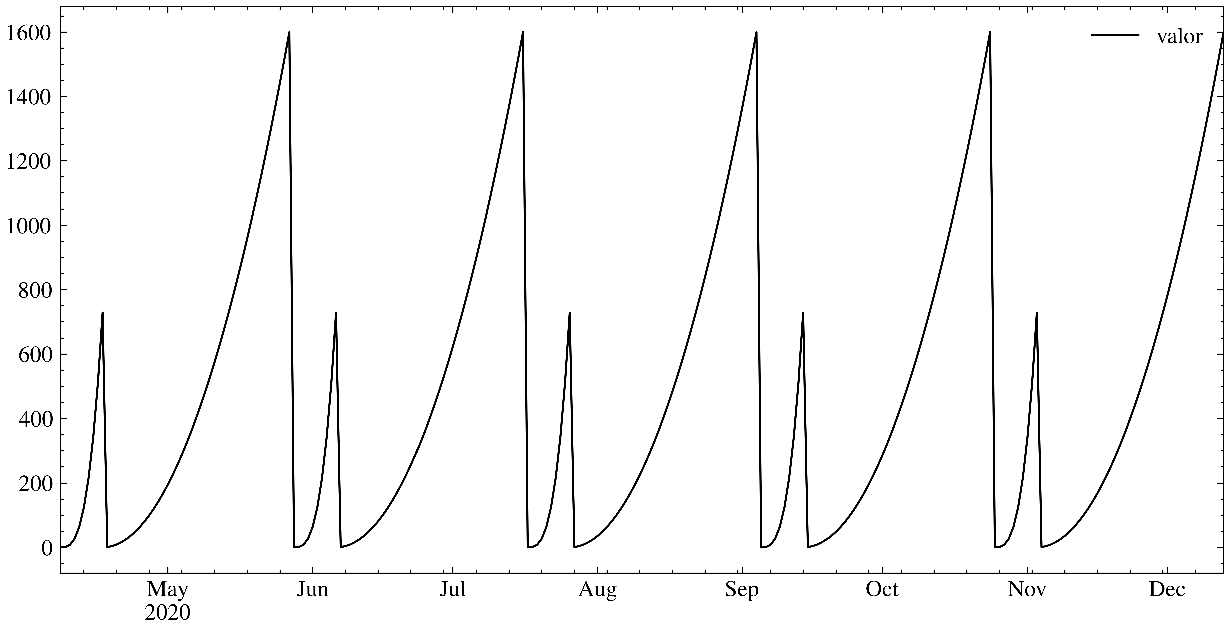
\includegraphics[width=5.0in]{img/seasonal_pattern.pdf}
    \caption{Componente de sazonalidade.}
    \label{fig:seasonal_pattern}
\end{figure}

O ruído é a parte do sinal que não possui valor semântico, ou seja, são distorções que ocorrem no sinal que podem ter como origem diversos fatores como o equipamento utilizado para fazer a coleta, erro humano, entre outros. Como nenhum sinal na vida real é livre de ruído, para aproximar a série temporal a de um problema real, foi adicionado um sinal de ruído branco gerado de forma pseudo-aleatória conforme apresentado na Figura~\ref{fig:noise}. Além do ruído, também foi adicionado um evento com impacto maior na série temporal com o objetivo de representar um fator inesperado na série. Esse fator pode ser equiparado a qualquer evento que possa alterar de forma disruptiva os dados observados na série temporal. Portanto, como a série possui uma tendência de crescimento, foi gerado um componente decrescente, ilustrado na Figura~\ref{fig:big_event}, nos últimos dias da série para ser somado aos outros componentes e gerar o efeito desejado.

\begin{figure}[!htp]
    \centering
    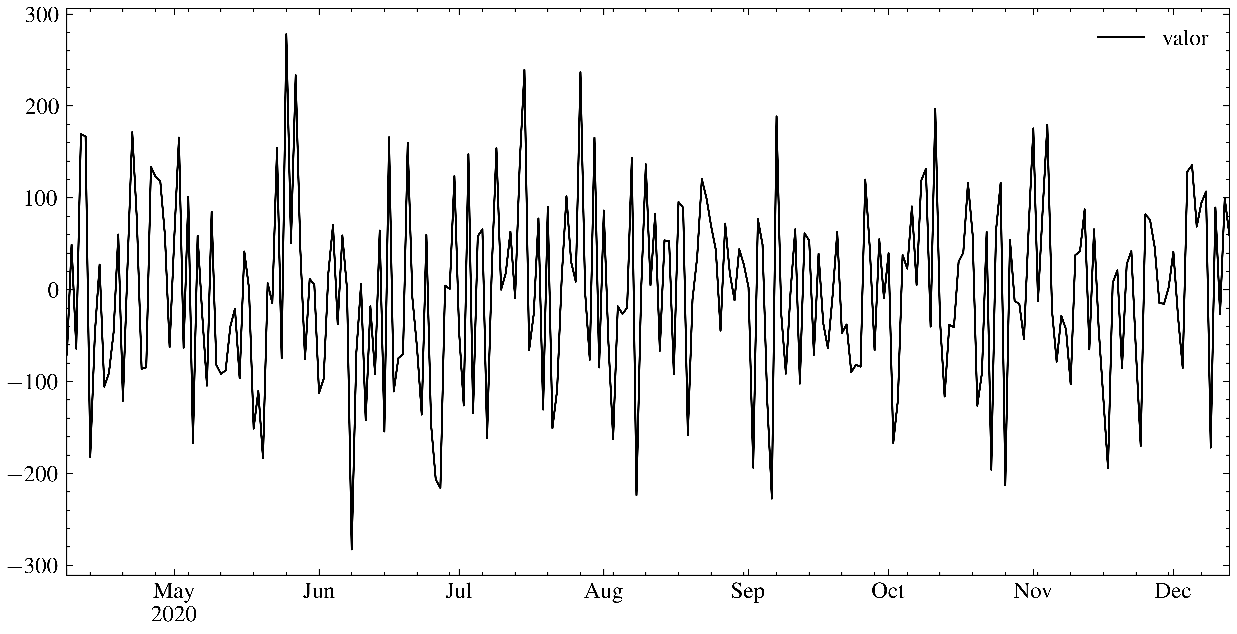
\includegraphics[width=5.0in]{img/noise.pdf}
    \caption{Ruído branco utilizado para compor a série temporal sintética.}
    \label{fig:noise}
\end{figure}

\begin{figure}[!htp]
    \centering
    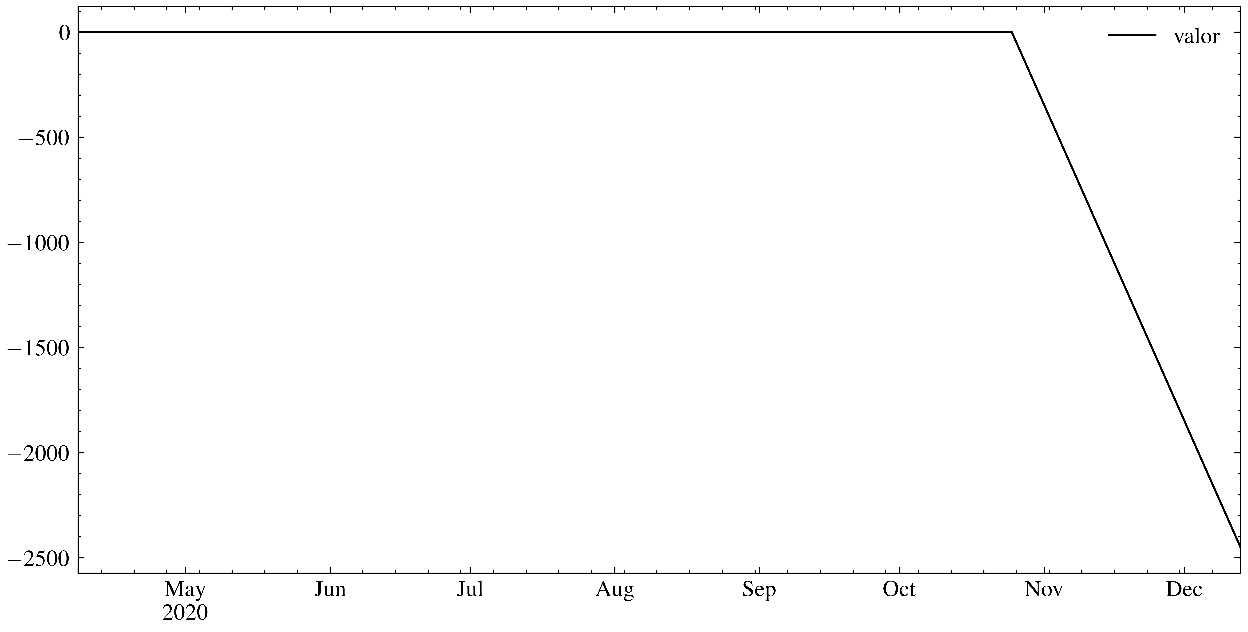
\includegraphics[width=5.0in]{img/big_event.pdf}
    \caption{Componente de evento inesperado descrescente.}
    \label{fig:big_event}
\end{figure}

Finalmente, após a soma de todos os componentes, é alcançada a série temporal resultante, conforme mostra a Figura~\ref{fig:dados_sinteticos}, onde será possível ajustar os modelos de predição e avaliar a capacidade de generalização de cada um. Como nas séries temporais anteriores, compartilha de flutuações de curto prazo, apesar de menores. Portanto, a Figura~\ref{fig:dados_sinteticos_ma} mostra as médias móveis calculadas com $W=4$ sobre a série temporal sintética. Esse valor foi escolhido na tentativa de suavizar as pequenas flutuações causadas propositalmente pela adição de ruído na composição da série temporal sintética.

\begin{figure}[!htp]
    \centering
    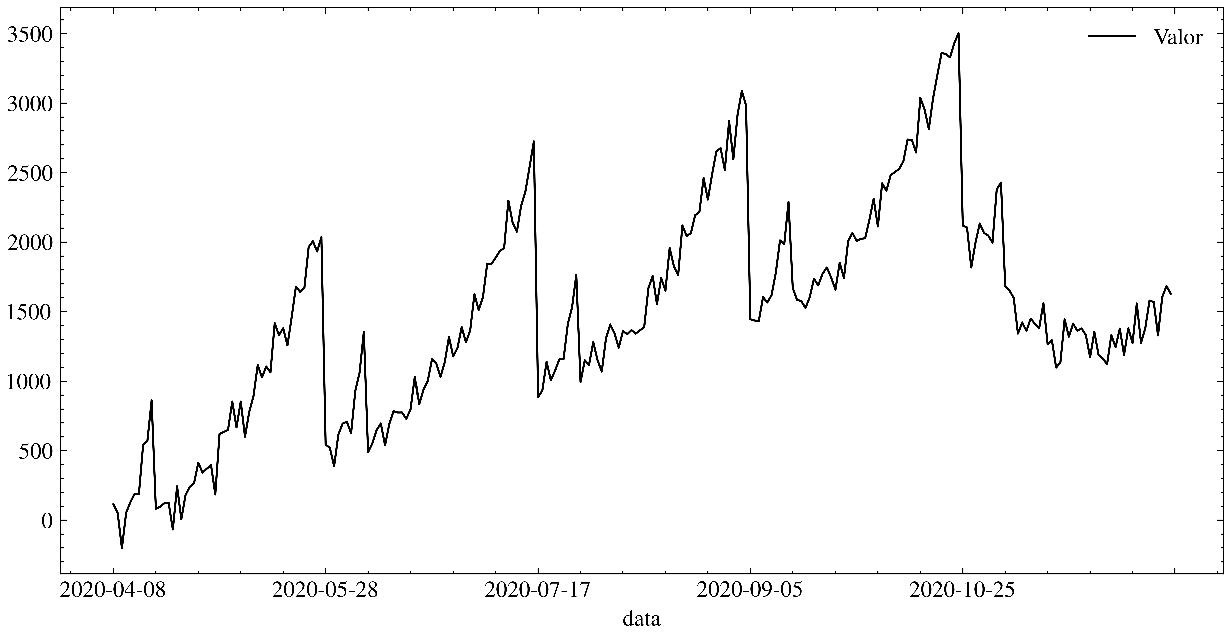
\includegraphics[width=5.0in]{img/dados_sinteticos.pdf}
    \caption{Série temporal gerada sinteticamente.}
    \label{fig:dados_sinteticos}
\end{figure}


\begin{figure}[!htp]
    \centering
    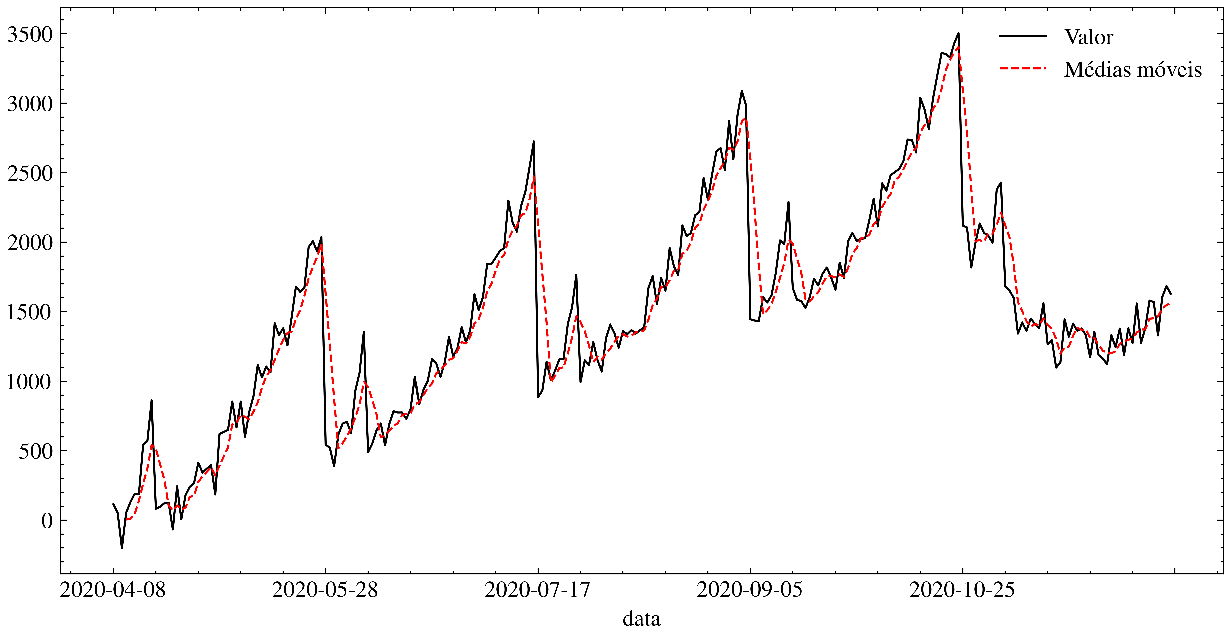
\includegraphics[width=5.0in]{img/dados_sinteticos_ma.pdf}
    \caption{Médias móveis da série temporal gerada sinteticamente.}
    \label{fig:dados_sinteticos_ma}
\end{figure}

\FloatBarrier

\section{Métricas de avaliação utilizadas}

Para a avaliação dos modelos preditivos, foram utilizadas 4 métricas de avaliação: \textit{Root Mean Square Error} (RMSE), \textit{Mean Absolute Error} (MAE), \textit{Mean Percentage Error} (MPE) e \textit{Mean Absolute Percentage Error} (MAPE). As métricas foram escolhidas com o objetivo de avaliar o erro de predição dos modelos de diferentes perspectivas. As Equações~\ref{eq:rmse}, \ref{eq:mae}, \ref{eq:mpe} e \ref{eq:mape} consideram $n$ como o número de observações presentes na coleção de dados, os valores de $y_{i}$ representam o conjunto de valores previstos pelos modelos e $x_{i}$ são os valores observados do conjunto separado para teste.

A Equação~\ref{eq:rmse} descreve o RMSE, que representa a raiz quadrada da média quadrática da diferença entre os valores previstos e observados. O RMSE é uma métrica que pode ser utilizada para comparar diferentes modelos ajustados e avaliados sobre um mesmo conjunto de dados, não sendo indicado para comparações entre coleções de dados diferentes. Esse comportamento é justificado pelo fato do RMSE ser uma métrica de acurácia que a escala depende da escala dos dados, como constatado em \cite{HYNDMAN2006679}. O valor de RMSE nunca assume valores negativos, e, em geral, valores menores são melhores que valores maiores. Esta métrica é sensível a erros muito grandes, ou seja, não possui um comportamento estável quando há \textit{outliers}.
\begin{equation} \label{eq:rmse}
    RMSE=\sqrt{\dfrac{\sum ^{n}_{i=1}\left( y_{i}-x_{i}\right) ^{2}}{n}}
\end{equation}

A métrica expressa pela Equação~\ref{eq:mae}, assim como o RMSE, é uma medida de acurácia. Com isso, compartilha da mesma propriedade de escala. A sua diferença principal, é que seu cálculo é linear, ou seja, as diferenças entre os valores observados e preditos são igualmente ponderadas na média.
\begin{equation} \label{eq:mae}
    MAE=\sum ^{n}_{i=1}\dfrac{\left| y_{i}-x_{i}\right| }{n}
\end{equation}

Diferente das métricas MAE, RMSE e MAPE, a \textit{Mean Percentage Error} (MPE), é uma métrica que considera o sinal do erro, ou seja, erros positivos e negativos se cancelam. Como consequência, a sua fórmula pode ser usada para medir o viés das predições. A Equação~\ref{eq:mpe} mostra como é feito o cáculo da MPE.
\begin{equation} \label{eq:mpe}
    MPE=\dfrac{1}{n}\sum ^{n}_{i=1}\dfrac{x_{i}-y_{i}}{x_{i}}
\end{equation}

A métrica \textit{Mean Absolute Percentage Error} (MAPE), é uma medida de acurácia, assim como a RMSE e MAE. Seu diferencial se dá pelo fato de ter uma interpretabilidade intuitiva comparado às outras métricas. Porém possui alguns defeitos bem conhecidos \cite{CHRISTOFALLIS2015}, como o erro da divisão por 0 e o fato de penalizar mais erros negativos do que erros positivos \cite{MAKRIDAKIS1993527}, levando à escolha de modelos cujo as predições são de valores mais baixos.


\begin{equation} \label{eq:mape}
    MAPE=\dfrac{1}{n}\sum ^{n}_{i=1}\left| \dfrac{y_{i}-x_{i}}{x_{i}}\right|
\end{equation}

\section{Resultados}
% apresentar formato de apresentação dos resultados.

\subsection{Avaliação por métricas}



\subsection{Tempos de execução}

\begin{table}[!htp]
    \caption{Tempo de ajuste dos modelos.}
    \setlength\extrarowheight{5pt}
    \begin{tabular}{|c|c|ccc|}
        \hline
        \rowcolor[HTML]{C0C0C0}
        \cellcolor[HTML]{C0C0C0}                          & \cellcolor[HTML]{C0C0C0}                          & \multicolumn{3}{c|}{\cellcolor[HTML]{C0C0C0}Dataset}                                                                                                                         \\ \cline{3-5}
        \rowcolor[HTML]{C0C0C0}
        \multirow{-2}{*}{\cellcolor[HTML]{C0C0C0}Modelo}  & \multirow{-2}{*}{\cellcolor[HTML]{C0C0C0}Métrica} & \multicolumn{1}{c|}{\cellcolor[HTML]{C0C0C0}Covid}                      & \multicolumn{1}{c|}{\cellcolor[HTML]{C0C0C0}Temperatura}               & Sintético                 \\ \hline
        \cellcolor[HTML]{C0C0C0}                          & RMSE                                              & \multicolumn{1}{c|}{779 ms ± 2.4 ms}                                    & \multicolumn{1}{c|}{3.61 s ± 5.34 ms}                                  & 38.4 ms ± 383 µs          \\ \cline{2-5}
        \rowcolor[HTML]{EFEFEF}
        \cellcolor[HTML]{C0C0C0}                          & MAPE                                              & \multicolumn{1}{c|}{\cellcolor[HTML]{EFEFEF}1.34 s ± 2.11ms}            & \multicolumn{1}{c|}{\cellcolor[HTML]{EFEFEF}3.61 s ± 4.68 ms}          & 38.3 ms ± 184 µs          \\ \cline{2-5}
        \cellcolor[HTML]{C0C0C0}                          & MAE                                               & \multicolumn{1}{c|}{779 ms ± 1.2 ms}                                    & \multicolumn{1}{c|}{3.61 s ± 8.5 ms}                                   & 38.4 ms ± 225 µs          \\ \cline{2-5}
        \rowcolor[HTML]{EFEFEF}
        \multirow{-4}{*}{\cellcolor[HTML]{C0C0C0}ARIMA}   & MPE                                               & \multicolumn{1}{c|}{\cellcolor[HTML]{EFEFEF}1.61 s ± 1.33 ms}           & \multicolumn{1}{c|}{\cellcolor[HTML]{EFEFEF}6.36 s ± 9.48 ms}          & 566 ms ± 705 µs           \\ \hline
        \cellcolor[HTML]{C0C0C0}                          & RMSE                                              & \multicolumn{1}{c|}{\textbf{4.41 ms ± 151 µs}}                          & \multicolumn{1}{c|}{\textbf{31.2 ms ± 526 µs}}                         & \textbf{9.97 ms ± 143 µs} \\ \cline{2-5}
        \rowcolor[HTML]{EFEFEF}
        \cellcolor[HTML]{C0C0C0}                          & MAPE                                              & \multicolumn{1}{c|}{\cellcolor[HTML]{EFEFEF}\textbf{4.46 ms ± 75.1 µs}} & \multicolumn{1}{c|}{\cellcolor[HTML]{EFEFEF}\textbf{19.5 ms ± 409 µs}} & \textbf{10.1 ms ± 166 µs} \\ \cline{2-5}
        \cellcolor[HTML]{C0C0C0}                          & MAE                                               & \multicolumn{1}{c|}{\textbf{8.65 ms ± 126 µs}}                          & \multicolumn{1}{c|}{\textbf{19.3 ms ± 149 µs}}                         & \textbf{10.5 ms ± 116 µs} \\ \cline{2-5}
        \rowcolor[HTML]{EFEFEF}
        \multirow{-4}{*}{\cellcolor[HTML]{C0C0C0}ReW}     & MPE                                               & \multicolumn{1}{c|}{\cellcolor[HTML]{EFEFEF}\textbf{4.41 ms ± 151 µs}}  & \multicolumn{1}{c|}{\cellcolor[HTML]{EFEFEF}\textbf{64.7 ms ± 549 µs}} & \textbf{8.86 ms ± 123 µs} \\ \hline
        \cellcolor[HTML]{C0C0C0}                          & RMSE                                              & \multicolumn{1}{c|}{56.5 ms ± 17.9 ms}                                  & \multicolumn{1}{c|}{205 ms ± 176 µs}                                   & 60.7 ms ± 87 µs           \\ \cline{2-5}
        \rowcolor[HTML]{EFEFEF}
        \cellcolor[HTML]{C0C0C0}                          & MAPE                                              & \multicolumn{1}{c|}{\cellcolor[HTML]{EFEFEF}46 ms ± 63.1 µs}            & \multicolumn{1}{c|}{\cellcolor[HTML]{EFEFEF}179 ms ± 514 µs}           & 60.9 ms ± 174 µs          \\ \cline{2-5}
        \cellcolor[HTML]{C0C0C0}                          & MAE                                               & \multicolumn{1}{c|}{44.6 ms ± 109 µs}                                   & \multicolumn{1}{c|}{180 ms ± 396 µs}                                   & 61.1 ms ± 177 µs          \\ \cline{2-5}
        \rowcolor[HTML]{EFEFEF}
        \multirow{-4}{*}{\cellcolor[HTML]{C0C0C0}Prophet} & MPE                                               & \multicolumn{1}{c|}{\cellcolor[HTML]{EFEFEF}46 ms ± 72.1 µs}            & \multicolumn{1}{c|}{\cellcolor[HTML]{EFEFEF}203 ms ± 200 µs}           & 68.1 ms ± 178 µs          \\ \hline
    \end{tabular}
\end{table}

\begin{table}[!htp]
    \caption{Tempo de inferência dos modelos.}
    \setlength\extrarowheight{5pt}
    \begin{tabular}{|c|c|ccc|}
        \hline
        \rowcolor[HTML]{C0C0C0}
        \cellcolor[HTML]{C0C0C0}                          & \cellcolor[HTML]{C0C0C0}                          & \multicolumn{3}{c|}{\cellcolor[HTML]{C0C0C0}Dataset}                                                                                                                         \\ \cline{3-5}
        \rowcolor[HTML]{C0C0C0}
        \multirow{-2}{*}{\cellcolor[HTML]{C0C0C0}Modelo}  & \multirow{-2}{*}{\cellcolor[HTML]{C0C0C0}Métrica} & \multicolumn{1}{c|}{\cellcolor[HTML]{C0C0C0}Covid}                      & \multicolumn{1}{c|}{\cellcolor[HTML]{C0C0C0}Temperatura}               & Sintético                 \\ \hline
        \cellcolor[HTML]{C0C0C0}                          & RMSE                                              & \multicolumn{1}{c|}{960 µs ± 2.51 µs}                                   & \multicolumn{1}{c|}{951 µs ± 14.4 µs}                                  & 1.92 ms ± 28.5 µs         \\ \cline{2-5}
        \rowcolor[HTML]{EFEFEF}
        \cellcolor[HTML]{C0C0C0}                          & MAPE                                              & \multicolumn{1}{c|}{\cellcolor[HTML]{EFEFEF}970 µs ± 1.83 µs}           & \multicolumn{1}{c|}{\cellcolor[HTML]{EFEFEF}942 µs ± 4.96 µs}          & 1.93 ms ± 33.3 µs         \\ \cline{2-5}
        \cellcolor[HTML]{C0C0C0}                          & MAE                                               & \multicolumn{1}{c|}{958 µs ± 2.81 µs}                                   & \multicolumn{1}{c|}{972 µs ± 8.09 µs}                                  & 1.92 ms ± 24.8 µs         \\ \cline{2-5}
        \rowcolor[HTML]{EFEFEF}
        \multirow{-4}{*}{\cellcolor[HTML]{C0C0C0}ARIMA}   & MPE                                               & \multicolumn{1}{c|}{\cellcolor[HTML]{EFEFEF}959 µs ± 5.72 µs}           & \multicolumn{1}{c|}{\cellcolor[HTML]{EFEFEF}956 µs ± 7.02 µs}          & 953 µs ± 27.8 µs          \\ \hline
        \cellcolor[HTML]{C0C0C0}                          & RMSE                                              & \multicolumn{1}{c|}{\textbf{142 µs ± 2.8 µs}}                           & \multicolumn{1}{c|}{\textbf{149 µs ± 349 ns}}                          & \textbf{330 µs ± 4.67}    \\ \cline{2-5}
        \rowcolor[HTML]{EFEFEF}
        \cellcolor[HTML]{C0C0C0}                          & MAPE                                              & \multicolumn{1}{c|}{\cellcolor[HTML]{EFEFEF}\textbf{87.6 µs ± 1.22 µs}} & \multicolumn{1}{c|}{\cellcolor[HTML]{EFEFEF}\textbf{106 µs ± 339 ns}}  & \textbf{494 µs ± 12.8 µs} \\ \cline{2-5}
        \cellcolor[HTML]{C0C0C0}                          & MAE                                               & \multicolumn{1}{c|}{\textbf{145 µs ± 2.3 µs}}                           & \multicolumn{1}{c|}{\textbf{107 µs ± 1.45 µs}}                         & \textbf{512 µs ± 7.91 µs} \\ \cline{2-5}
        \rowcolor[HTML]{EFEFEF}
        \multirow{-4}{*}{\cellcolor[HTML]{C0C0C0}ReW}     & MPE                                               & \multicolumn{1}{c|}{\cellcolor[HTML]{EFEFEF}\textbf{91 µs ± 638 ns}}    & \multicolumn{1}{c|}{\cellcolor[HTML]{EFEFEF}\textbf{232 µs ± 6.43 µs}} & \textbf{422 µs ± 8.16 µs} \\ \hline
        \cellcolor[HTML]{C0C0C0}                          & RMSE                                              & \multicolumn{1}{c|}{1.26 s ± 10.7 ms}                                   & \multicolumn{1}{c|}{1.88 s ± 3.79 ms}                                  & 898 ms ± 768 µs           \\ \cline{2-5}
        \rowcolor[HTML]{EFEFEF}
        \cellcolor[HTML]{C0C0C0}                          & MAPE                                              & \multicolumn{1}{c|}{\cellcolor[HTML]{EFEFEF}1.25 s ± 1.59 ms}           & \multicolumn{1}{c|}{\cellcolor[HTML]{EFEFEF}2.13 s ± 711 µs}           & 906 ms ± 600 µs           \\ \cline{2-5}
        \cellcolor[HTML]{C0C0C0}                          & MAE                                               & \multicolumn{1}{c|}{1.25 s ± 1.29 ms}                                   & \multicolumn{1}{c|}{2.13 s ± 940 µs}                                   & 898 ms ± 753 µs           \\ \cline{2-5}
        \rowcolor[HTML]{EFEFEF}
        \multirow{-4}{*}{\cellcolor[HTML]{C0C0C0}Prophet} & MPE                                               & \multicolumn{1}{c|}{\cellcolor[HTML]{EFEFEF}1.25 s ± 1.26 ms}           & \multicolumn{1}{c|}{\cellcolor[HTML]{EFEFEF}1.88 s ± 530 µs}           & 899 ms ± 1.24 ms          \\ \hline
    \end{tabular}
\end{table}

\FloatBarrier

\subsection{Uso de memória}

\begin{table}[!htp]
    \caption{Uso de memória de cada modelo por métrica otimizada e dataset.}
    \setlength\extrarowheight{5pt}
    \centering
    \begin{tabular}{|c|c|ccc|}
        \hline
        \rowcolor[HTML]{C0C0C0}
        \cellcolor[HTML]{C0C0C0}                          & \cellcolor[HTML]{C0C0C0}                          & \multicolumn{3}{c|}{\cellcolor[HTML]{C0C0C0}Dataset}                                                                                                   \\ \cline{3-5}
        \rowcolor[HTML]{C0C0C0}
        \multirow{-2}{*}{\cellcolor[HTML]{C0C0C0}Modelo}  & \multirow{-2}{*}{\cellcolor[HTML]{C0C0C0}Métrica} & \multicolumn{1}{c|}{\cellcolor[HTML]{C0C0C0}Covid}              & \multicolumn{1}{c|}{\cellcolor[HTML]{C0C0C0}Temperatura}        & Sintético          \\ \hline
        \cellcolor[HTML]{C0C0C0}                          & RMSE                                              & \multicolumn{1}{c|}{9.086 MiB}                                  & \multicolumn{1}{c|}{43.621 MiB}                                 & 3.105 MiB          \\ \cline{2-5}
        \rowcolor[HTML]{EFEFEF}
        \cellcolor[HTML]{C0C0C0}                          & MAPE                                              & \multicolumn{1}{c|}{\cellcolor[HTML]{EFEFEF}11.383 MiB}         & \multicolumn{1}{c|}{\cellcolor[HTML]{EFEFEF}43.699 MiB}         & 3.078 MiB          \\ \cline{2-5}
        \cellcolor[HTML]{C0C0C0}                          & MAE                                               & \multicolumn{1}{c|}{8.816 MiB}                                  & \multicolumn{1}{c|}{44.035 MiB}                                 & 3.359 MiB          \\ \cline{2-5}
        \rowcolor[HTML]{EFEFEF}
        \multirow{-4}{*}{\cellcolor[HTML]{C0C0C0}ARIMA}   & MPE                                               & \multicolumn{1}{c|}{\cellcolor[HTML]{EFEFEF}13.734 MiB}         & \multicolumn{1}{c|}{\cellcolor[HTML]{EFEFEF}50.805 MiB}         & 6.457 MiB          \\ \hline
        \cellcolor[HTML]{C0C0C0}                          & RMSE                                              & \multicolumn{1}{c|}{\textbf{0.512 MiB}}                         & \multicolumn{1}{c|}{\textbf{1.039 MiB}}                         & \textbf{0.598 MiB} \\ \cline{2-5}
        \rowcolor[HTML]{EFEFEF}
        \cellcolor[HTML]{C0C0C0}                          & MAPE                                              & \multicolumn{1}{c|}{\cellcolor[HTML]{EFEFEF}\textbf{0.000 MiB}} & \multicolumn{1}{c|}{\cellcolor[HTML]{EFEFEF}\textbf{0.922 MiB}} & \textbf{0.570 MiB} \\ \cline{2-5}
        \cellcolor[HTML]{C0C0C0}                          & MAE                                               & \multicolumn{1}{c|}{\textbf{0.586 MiB}}                         & \multicolumn{1}{c|}{\textbf{0.887 MiB}}                         & \textbf{0.898 MiB} \\ \cline{2-5}
        \rowcolor[HTML]{EFEFEF}
        \multirow{-4}{*}{\cellcolor[HTML]{C0C0C0}ReW}     & MPE                                               & \multicolumn{1}{c|}{\cellcolor[HTML]{EFEFEF}\textbf{0.645 MiB}} & \multicolumn{1}{c|}{\cellcolor[HTML]{EFEFEF}\textbf{0.809 MiB}} & \textbf{0.562 MiB} \\ \hline
        \cellcolor[HTML]{C0C0C0}                          & RMSE                                              & \multicolumn{1}{c|}{90.676 MiB}                                 & \multicolumn{1}{c|}{101.699 MiB}                                & 89.719 MiB         \\ \cline{2-5}
        \rowcolor[HTML]{EFEFEF}
        \cellcolor[HTML]{C0C0C0}                          & MAPE                                              & \multicolumn{1}{c|}{\cellcolor[HTML]{EFEFEF}90.652 MiB}         & \multicolumn{1}{c|}{\cellcolor[HTML]{EFEFEF}102.074 MiB}        & 89.203 MiB         \\ \cline{2-5}
        \cellcolor[HTML]{C0C0C0}                          & MAE                                               & \multicolumn{1}{c|}{90.621 MiB}                                 & \multicolumn{1}{c|}{102.273 MiB}                                & 89.426 MiB         \\ \cline{2-5}
        \rowcolor[HTML]{EFEFEF}
        \multirow{-4}{*}{\cellcolor[HTML]{C0C0C0}Prophet} & MPE                                               & \multicolumn{1}{c|}{\cellcolor[HTML]{EFEFEF}90.617 MiB}         & \multicolumn{1}{c|}{\cellcolor[HTML]{EFEFEF}101.926 MiB}        & 89.277 MiB         \\ \hline
    \end{tabular}
\end{table}

\FloatBarrier

\subsection{Discussão}
